\chapter{Decomposition Approach Evaluation}
\label{appendix:decompositionAppraoches}

During early feasibility tests with graph clustering, we encountered significant problems as documented in the next Section. As consequence of these results, we conducted a feasibility assessment with a professor of mathematics on the graph based approach, documented in Appendix \ref{sec:feasibilityAssessment}. Out of the feasibility assessment, two additional approaches on how the Service Cutter can solve the decomposition problem were defined and are discussed in this Chapter. Nevertheless, the conclusion Section states how challenges in these approaches and further research on clustering graphs led us back to follow the graph based approach.

\section{Graph Clustering Problems}

At first, the clustering algorithm evaluated documented in Appendix \ref{appendix:graphClustering} did not contain the Leung algorithm as this has been found later during the project. The two candidate algorithms were MCL and Girvan-Newman. We did a feasibility test using a small Booking System sample containing three entities:

\begin{description}
	\item[Customer Entity] containing address, accountNr, creditCardNr, and name.
	\item[Article Entity] containing articleName, price, and serial.
	\item[Booking Entity] containing stotalPrice, paymentDate, bookingDate, and bookingState.
\end{description}

\begin{figure}[H]
	\begin{center}
		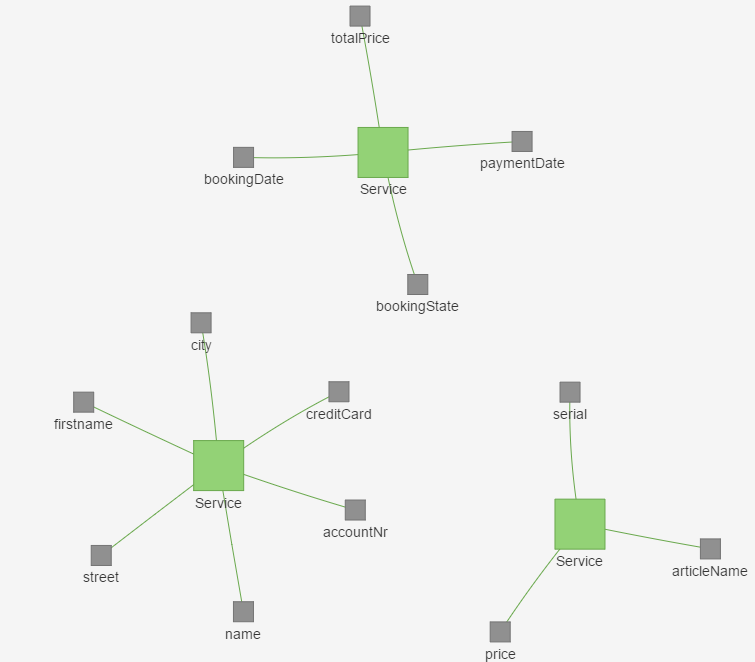
\includegraphics[scale=0.75]{images/booking_entities.png}
	\end{center}
	\caption{Expected output for Booking Example}
	\label{fig:bookingExample}
\end{figure}

To keep the sample simple we only added information for the \textit{Lifecycle \& Identity Commonality} criterion, so that the output is expected to show exactly the entity borders as shown in Figure \ref{fig:bookingExample}.


\begin{figure}[H]
	\begin{center}
		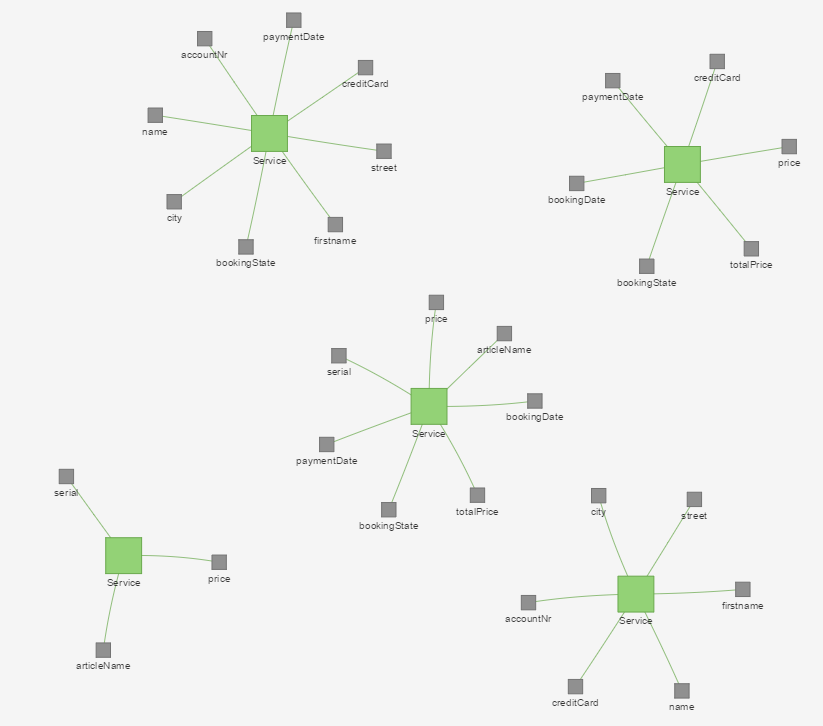
\includegraphics[scale=0.7]{images/booking_entities_mcl.png}
	\end{center}
	\caption{Booking Example with the MCL algorithm}
	\label{fig:bookingExampleMCL}
\end{figure}

The MCL algorithm's result for this example are shown in Figure \ref{fig:bookingExampleMCL}. Obviously this does not match the expectations. Nanoentities are attached to multiple services. Another MCL implementation (TODO), also provided within the Gephi platform, did not contain duplicate nanoentities but therefore missed attaching every nanoentity to a service. Both implementations do not meet the \textit{distinct clusters} requirement that a nanoentity should be assigned to one and only one service. 

The distinct clusters requirement is satisfied by the original MCL implementation written in R, so that the problems can be identified as implementation problem. A solution to this problem would be to write a Java wrapper for the R implementation as described in Section XXX. %TODO Future Work)

\begin{figure}[H]
	\begin{center}
		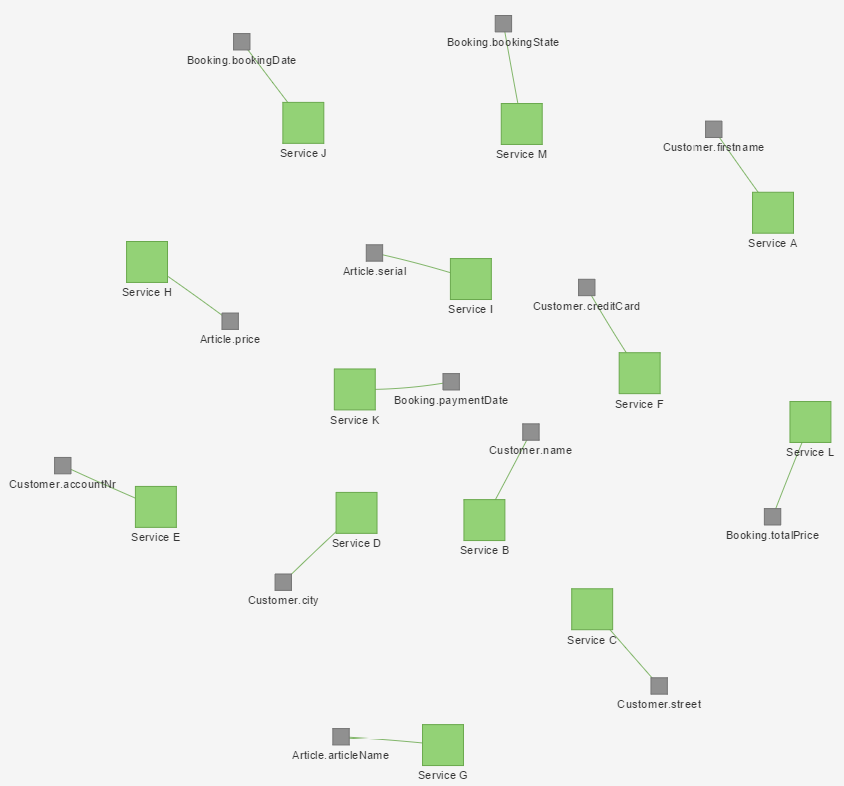
\includegraphics[scale=0.65]{images/girvan_entities_fail.png}
	\end{center}
	\caption{Booking Example with the Girven-Newman algorithm}
	\label{fig:bookingExampleGirvan}
\end{figure}

Figure \ref{fig:bookingExampleGirvan} shows the unsatisfying result provided by Girvan-Newman. By reasons of these unexpected results, we consulted a professor of mathematics as documented in Appendix \ref{sec:feasibilityAssessment} which lead to the alternative approaches described in the next Sections.

\section{Approach \#2: Rating of Possible Service Cuts}

The idea this approach introduces is to create a set of all possible service cuts and rate the cuts isolated per coupling criteria. The approach is illustrated in Figure \ref{fig:setProcess}.

%TODO update Data Fields to NanoEntities, Processor to Scorer
\begin{figure}[H]
	\begin{center}
		\includegraphics[scale=0.45]{diagrams/scoring_process.png}
	\end{center}
	\caption{Approach \#2: Set Rating}
	\label{fig:setProcess}
\end{figure}

This approach is processed in three steps:

\begin{description}
	\item[Partitioning] Based on the nanoentities, a set of all possible candidate service cuts is calculated. This includes every theoretically possible service cut for every number of services. For practical usage, this step needs to be optimized. 
	\item[Assessment] For all coupling criteria a processor assesses all service cuts with a score describing how well the criteria's requirements are met. The score is a number between 0 and 10, while 10 implies that all requirements are perfectly satisfied. 
	\item[Evaluation] The user optionally defines priorities how important each criteria is for his system. The priorities are defined with approximately exponential numbers like the Fibonacci sequence. These priorities are applied on the service cut scores. The resulting best candidate cut is then presented to the user.
\end{description}

\subsection{Discussion}

An advantage of this approach is that each relevant step is clearly separated and can thus be analyzed, debugged and visualized better than in the graph based approach. The assessment and score calculation is done separately for every cut and for every coupling criteria. Each criteria scorer scores candidate cuts with a uniform scoring range. As solutions do not need to be constructed but only rated, the single dimensionality problem described in Section \ref{subsec:singleDimensionality} does not apply.

The weak point is the partitioning process. Theoretically every possible set of services where each nanoentity is contained in one and only one service is a candidate cut. In mathematics this is described as the \textit{partition of a set}\cite{partitionOfASet} problem. The Bell number $B_n$ defines the amount of possible partitions: 


\begin{displaymath}
B_{n+1}=\sum_{j=0}^n {n\choose j} B_j
\end{displaymath}

For the Service Cutter, $n$ is the number of nanoentities. The number of possible service cuts for $n=20$ nanoentities is $51'724'158'235'372$\footnote{We do not print the number for the required $2000$ nanoentities for lack of space in this document.}.

The Bell number includes cuts for $1 - n$ number of services. In the context of a software system only certain numbers of services are realistic. The \textit{Stirling numbers of the second kind} calculate the Bell number for a given number of sets $k$:

\begin{displaymath}
\left\{ {n \atop k}\right\} = \frac{1}{k!}\sum_{j=0}^{k} (-1)^{k-j} \binom{k}{j} j^n
\end{displaymath}

For $n=20$ nanoentities and $k=4$ services the equation results in $45'232'115'901$ possible cuts. For $k=6$ the result is $4'306'078'895'384$.

During a discussion with our industry partner and supervisor documented in Appendix \ref{sec:status22102015}, we decided that the Service Cutter should be able to process system models with up to 2000 nanoentities. We therefore concluded in the same meeting that this approach is not practicable without a heuristic approach of finding a small set of relevant candidate cuts. 

A possible heuristic approach is to take into account one or a few coupling criteria information about the system to find service candidates. A simple example would be to only analyze cuts where nanoentities of the same entity are not split across services so that only entities and not it's nanoentities need to be considered.

As we tried to find a heuristic approach to calculate candidate cuts, we discovered a new idea for the composition algorithm described in the next Section. 

\section{Approach \#3: Constructing Services - a Heuristic Approach}

(Notes only)
Idee:

Distanzkriterien: Umso mehr Services umso besser die Lösung (Nanoservices)
Nähekriterien: Umso weniger Services umso besser die Lösung (Monolith)

Die richtige Anzahl Services ist eine kritische Dimension der Lösung, welche unter anderem aber von vielen externen (z.B Infrastruktur) Faktoren abhängt. Entscheidung: Die Verantwortung für das bestimmen der Anzahl Services an den User auslagern.

Nun ist es möglich eine bestimmte Anzahl Services zu füllen. Dazu kann ein heuristischer, empirischer Algorithmus mit intelligentem Rütteln genommen werden. 
Jede Verbindung von zwei Feldern wird von jedem CC mit einer einheitlichen Einheit bewertet. Dadurch kann einfach bestummen werden, wie gut ein Feld in ein Topf passt. Alle Töpfe werden gefüllt (wenn es nirgends passt in den kleinsten Topf). Danach wird angefangen Feldern die am wenigsten passen in einen anderen Topf zu werfen.
Der Algorithmus kann beliebig(?) weiterlaufen und optimieren. Wenn der Algorithmus gut funktioniert, kann man während der Optimierung auch die Gewichtung anpassen und schauen was damit passiert.
Idee: Snapshots machen von Status bevor eine Gewichtung angepasst wird.
Idee: Am Anfang 5 Minuten durchlaufen, 10 Vorschläge ausarbeiten und dann den user entscheiden lassen auf welchen er weiter optimieren will (?) Evtl. kann auch der Algorithmus entscheiden indem er die lösungen vergleicht? 

Weitere Idee: Aufsplitten auf logische (A) und physische (B) Kriterien und Decomposition mode? Kann der Algorithmus in zwei Schritten geschehen? Bzw. lösen wir eigentlich 2 Probleme (Logisch \& Physisch) auf einmal?

\subsection{Conclusion}